% Created 2022-06-03 Fri 21:24
% Intended LaTeX compiler: pdflatex
\documentclass[twoside, twocolumn, 9pt, draft]{article}
\usepackage[utf8]{inputenc}
\usepackage[T1]{fontenc}
\usepackage{graphicx}
\usepackage{longtable}
\usepackage{wrapfig}
\usepackage{rotating}
\usepackage[normalem]{ulem}
\usepackage{amsmath}
\usepackage{amssymb}
\usepackage{capt-of}
\usepackage{hyperref}

\usepackage{abstract}%% easy abstract environment (from frontmatter pkg "ltxfront")
\usepackage[export]{adjustbox}%% expanded control over image, minipages, etc
\usepackage{sectsty}%% control of section heading appearance in default and script doc classes
\usepackage{setspace}%% implements \setstretch for line spacing
\usepackage{amsthm}%% formal mathematics environments
\usepackage{mathtools}%% bugfixing and additional tools for amsmath
\usepackage{lastpage}%% allows ref to lastpage
\usepackage{amsfonts}%% formal math fonts
\usepackage{mathptmx}%% ghostscript/postscript fonts and font loading options
\usepackage{charter}%% ghostscript/postscript fonts outside of math envs
\usepackage{times}%% more ghostscript/postscript
\usepackage{bm}%% bold math
\usepackage[%% full (expands on capt-of) control over appearance of float captions
%margin=10pt
format=plain,
justification=justified,
singlelinecheck=false,
font={small, sf},
labelfont=bf,
labelsep=space
]{caption}%% global preamble, use \captionsetup{} to config env)

\usepackage[compact]{titlesec}%% replacement of sectioning macros, coexsiting with old stuff
\usepackage{fancyhdr}%% improved headers and footers
\usepackage{fnpos}%% footnote positioning tools
\usepackage{sidecap}%% control of figure and caption positioning and margin spill
\usepackage{gensymb}%% inter-environment consistent measurment unit symbols
\usepackage{upgreek}%% easy lower and uppercase nonitalicized greek letters
\usepackage{soul}%% spaceout and underline macros

\usepackage{array}%% modernization of array and tabular envs
\usepackage{droidsans}%% use android sanserif fonts...

\usepackage[usenames,dvipsnames]{xcolor}%% text color macros
\usepackage[version=3]{mhchem}%% for writing chemical formulae
\usepackage[super,sort&compress,comma]{natbib}%% prefered citation engine

%% control margin configurations and visualize framing
\usepackage[%%rsc page standard follows
left=1.5cm,
right=1.5cm,
top=1.785cm,
bottom=2.0cm
]{geometry}

\addto{\captionsenglish}{%
\renewcommand{\refname}{Notes and references}
}

\definecolor{cream}{RGB}{222,217,201}%% required for use of rsc frontmatter

%\usepackage[mathlines]{lineno}%% Enable numbering of text and display math
%\linenumbers\relax%% Commence numbering lines
\date{\today}
\title{A High-Throughput Computational Dataset of Halide Perovskite Alloys\textsuperscript{\dag}}
\hypersetup{
 pdfauthor={Panayotis Manganaris},
 pdftitle={A High-Throughput Computational Dataset of Halide Perovskite Alloys\textsuperscript{\dag}},
 pdfkeywords={},
 pdfsubject={},
 pdfcreator={Emacs 29.0.50 (Org mode 9.5.3)}, 
 pdflang={English}}
\begin{document}

% Royal Society of Chemistry frontmatter conventions for quick recall via INCLUDE keyword

\pagestyle{fancy}
\thispagestyle{plain}
\fancypagestyle{plain}{
%%%HEADER%%%
\renewcommand{\headrulewidth}{0pt}
}
%%%END OF HEADER%%%

%%%PAGE SETUP - Please do not change any commands within this section%%%
\makeFNbottom
\makeatletter
\renewcommand\LARGE{\@setfontsize\LARGE{15pt}{17}}
\renewcommand\Large{\@setfontsize\Large{12pt}{14}}
\renewcommand\large{\@setfontsize\large{10pt}{12}}
\renewcommand\footnotesize{\@setfontsize\footnotesize{7pt}{10}}
\makeatother

\renewcommand{\thefootnote}{\fnsymbol{footnote}}
\renewcommand\footnoterule{\vspace*{1pt}% 
\color{cream}\hrule width 3.5in height 0.4pt \color{black}\vspace*{5pt}} 
\setcounter{secnumdepth}{5}

\makeatletter 
\renewcommand\@biblabel[1]{#1}            
\renewcommand\@makefntext[1]{\noindent\makebox[0pt][r]{\@thefnmark\,}#1}
\makeatother 
\renewcommand{\figurename}{\small{Fig.}~}
\sectionfont{\sffamily\Large}
\subsectionfont{\normalsize}
\subsubsectionfont{\bf}
\setstretch{1.125}
\setlength{\skip\footins}{0.8cm}
\setlength{\footnotesep}{0.25cm}
\setlength{\jot}{10pt}
\titlespacing*{\section}{0pt}{4pt}{4pt}
\titlespacing*{\subsection}{0pt}{15pt}{1pt}
%%%END OF PAGE SETUP%%%

%%%FOOTER%%%
\fancyfoot{}
\fancyfoot[LO,RE]{\vspace{-7.1pt}\includegraphics[height=9pt]{head_foot/LF}}
\fancyfoot[CO]{\vspace{-7.1pt}\hspace{13.2cm}\includegraphics{head_foot/RF}}
\fancyfoot[CE]{\vspace{-7.2pt}\hspace{-14.2cm}\includegraphics{head_foot/RF}}
\fancyfoot[RO]{\footnotesize{\sffamily{1--\pageref{LastPage} ~\textbar  \hspace{2pt}\thepage}}}
\fancyfoot[LE]{\footnotesize{\sffamily{\thepage~\textbar\hspace{3.45cm} 1--\pageref{LastPage}}}}
\fancyhead{}
\renewcommand{\headrulewidth}{0pt} 
\renewcommand{\footrulewidth}{0pt}
\setlength{\arrayrulewidth}{1pt}
\setlength{\columnsep}{6.5mm}
\setlength\bibsep{1pt}
%%%END OF FOOTER%%%

%%%FIGURE SETUP - please do not change any commands within this section%%%
\makeatletter 
\newlength{\figrulesep} 
\setlength{\figrulesep}{0.5\textfloatsep} 

\newcommand{\topfigrule}{\vspace*{-1pt}% 
\noindent{\color{cream}\rule[-\figrulesep]{\columnwidth}{1.5pt}} }

\newcommand{\botfigrule}{\vspace*{-2pt}% 
\noindent{\color{cream}\rule[\figrulesep]{\columnwidth}{1.5pt}} }

\newcommand{\dblfigrule}{\vspace*{-1pt}% 
\noindent{\color{cream}\rule[-\figrulesep]{\textwidth}{1.5pt}} }

\makeatother
%%%END OF FIGURE SETUP%%%

%%%TITLE, AUTHORS AND ABSTRACT%%%
\twocolumn[
\begin{@twocolumnfalse}
{%\includegraphics[height=30pt]{head_foot/journal_name}\hfill\raisebox{0pt}[0pt][0pt]{\includegraphics[height=55pt]{head_foot/RSC_LOGO_CMYK}}\\[1ex]
%\includegraphics[width=18.5cm]{head_foot/header_bar}}\par
\vspace{1em}
\sffamily
\begin{tabular}{m{4.5cm} p{13.5cm} }
%\includegraphics{head_foot/DOI}
& \noindent\LARGE{\textbf{A High-Throughput Computational Dataset of Halide Perovskite Alloys\textsuperscript{\dag}}}\\%
%Article title goes here
\vspace{0.3cm} & \vspace{0.3cm} \\
& \noindent\large{Jiaqi Yang\textsuperscript{a}, Panayotis Manganaris\textsuperscript{a}, and Arun Mannodi-Kanakkithodi\textsuperscript{a}}}\\
%Author names go here
\end{tabular}
\begin{abstract}
Novel halide Perovskites with improved stability and optoelectronic properties can be designed via composition engineering at cation and/or
anion sites. Data-driven methods, especially high-throughput first principles computations and subsequent analysis based on unique materials
descriptors, are key to achieving this goal. In this work, we report a Density Functional Theory (DFT) based dataset of 550 ABX\textsubscript{3} halide
Perovskite compounds, with various atomic and molecular species considered at A, B and X sites, and different amounts of mixing considered
at each site generated using the Special Quasirandom Structures (SQS) algorithm for alloys. We perform GGA-PBE calculations on pseudo-cubic
Perovskite structures to determine their lattice constants, stability in terms of formation and decomposition energies, electronic band gaps,
and properties extracted from optical absorption spectra. To elucidate the importance of the level of theory used, we further perform 300 calculations
using the more expensive HSE06 functional and determine lattice constant, stability and band gap, and compare PBE and HSE06 properties with
some experimentally measured results. Trends in the datasets are unraveled in terms of the effects of mixing at different sites, the
composition in terms of specific atomic or molecular species, and averaged elemental properties of species at different sites. This work
presents the most comprehensive DFT perovskite alloy dataset to date and the data, which is open-source, can be exploited to train
predictive and optimization models for accelerating the design of completely new compositions that may yield large solar cell efficiencies
and improved performance across many optoelectronic applications.
\end{abstract}
\end{@twocolumnfalse}
\vspace{0.6cm}
]
%%%END OF TITLE, AUTHORS AND ABSTRACT%%%

%%%FONT SETUP - please do not change any commands within this section
\renewcommand*\rmdefault{bch}\normalfont\upshape
\rmfamily
\section*{}
\vspace{-1cm}

%INCLUDE -- notice abstract is contained in titleblock

\footnotetext{\textsuperscript{a}School of Materials Engineering, Purdue University, West Lafayette, IN 47907, USA; E-mail: amannodi@purdue.edu}
\footnotetext{\textsuperscript{\dag}Electronic Supplementary Information (ESI) available: https://www.github.com/PanayotisManganaris/REPO_TODO. See DOI: 00.0000/00000000.}

\section*{Introduction}
\label{sec:orgb1819d1}
The challenge of optimizing Perovskite performance is one with many
facets. Almost every detail of a Perovskite crystal's structure and
chemistry effects its performance as a semiconductor. The size of the
unit cell effects its substrate affinity and in turn its carrier
concentrations. The crystal phase effects many aspects of the
electronic structure, including the band gap and optical response. Of
course, the structure is ultimately dependent on the proportions and
arrangement of the constituent elements.

\begin{figure*}
\centering
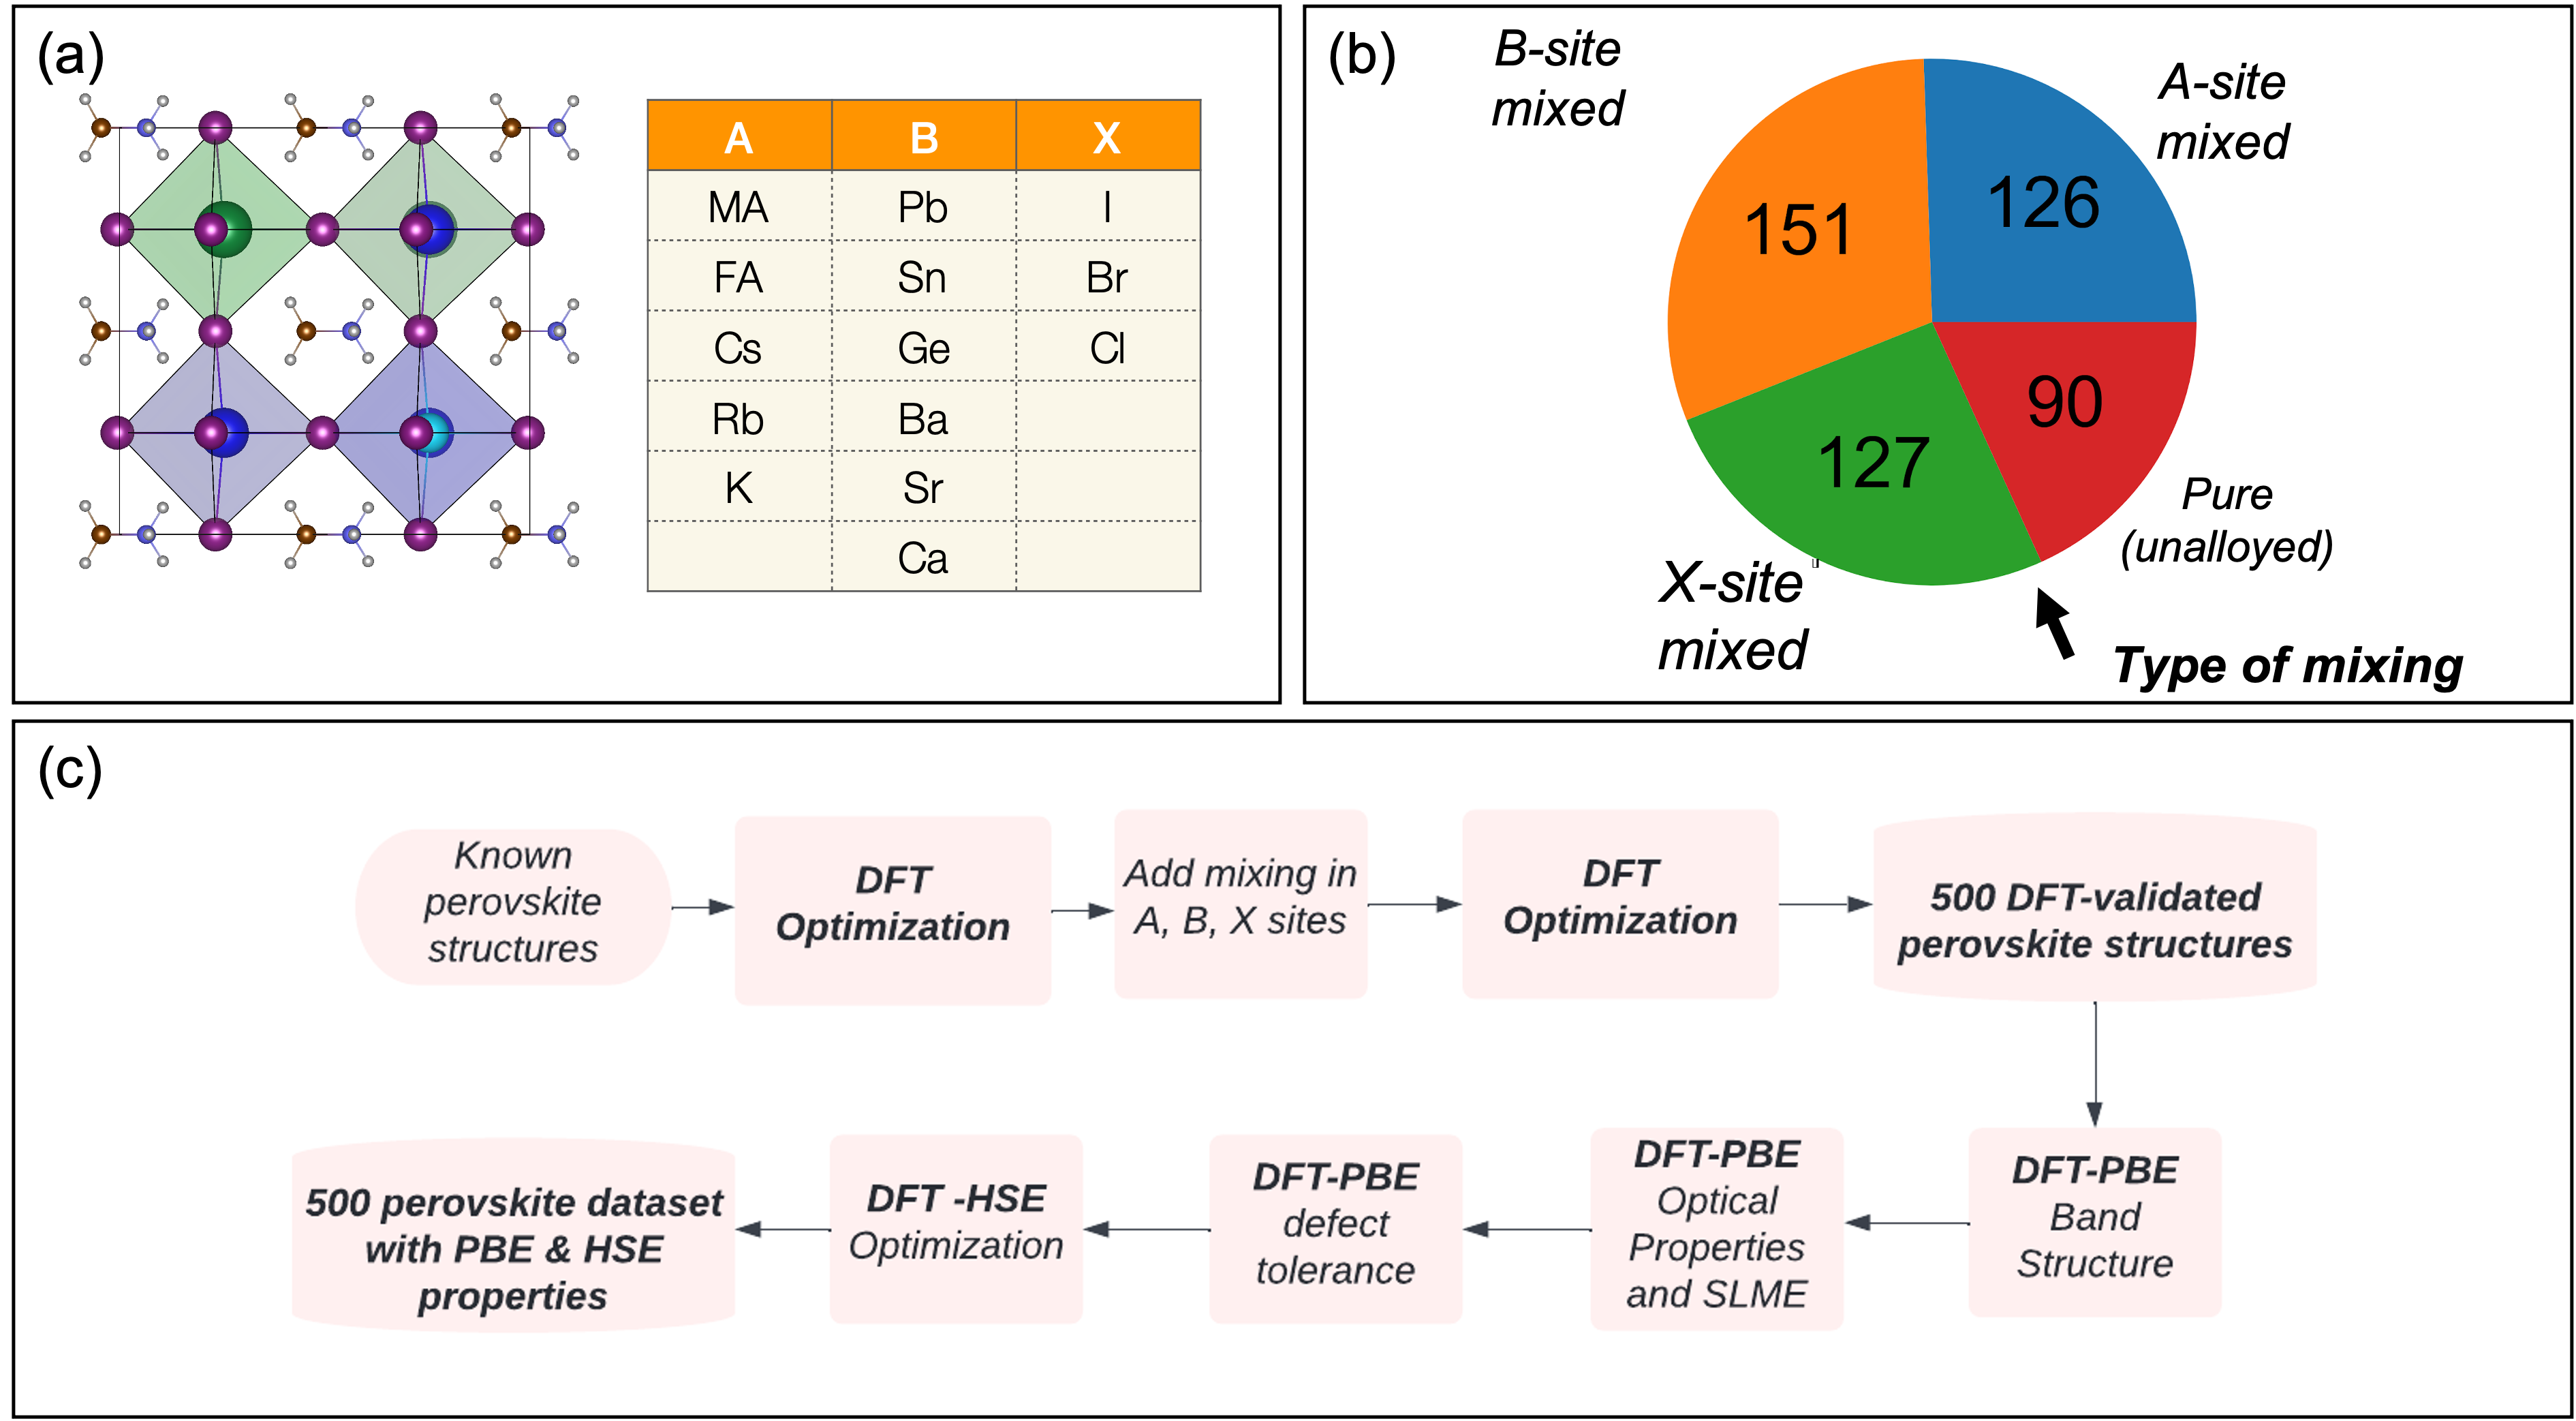
\includegraphics[h,width=.9\linewidth]{Figure1.png}
\caption{\label{Fig:outline} (a) Chemical space of ABX\textsubscript{3} perovskites. (b) Pie charts showing the amounts of various atomic and molecular species as well as types of mixing in the DFT dataset. (c) Detailed outline of this work.}
\end{figure*}

\subsection*{Coverage of Chemical Space}
\label{sec:orgd64070f}

\begin{figure*}
\centering
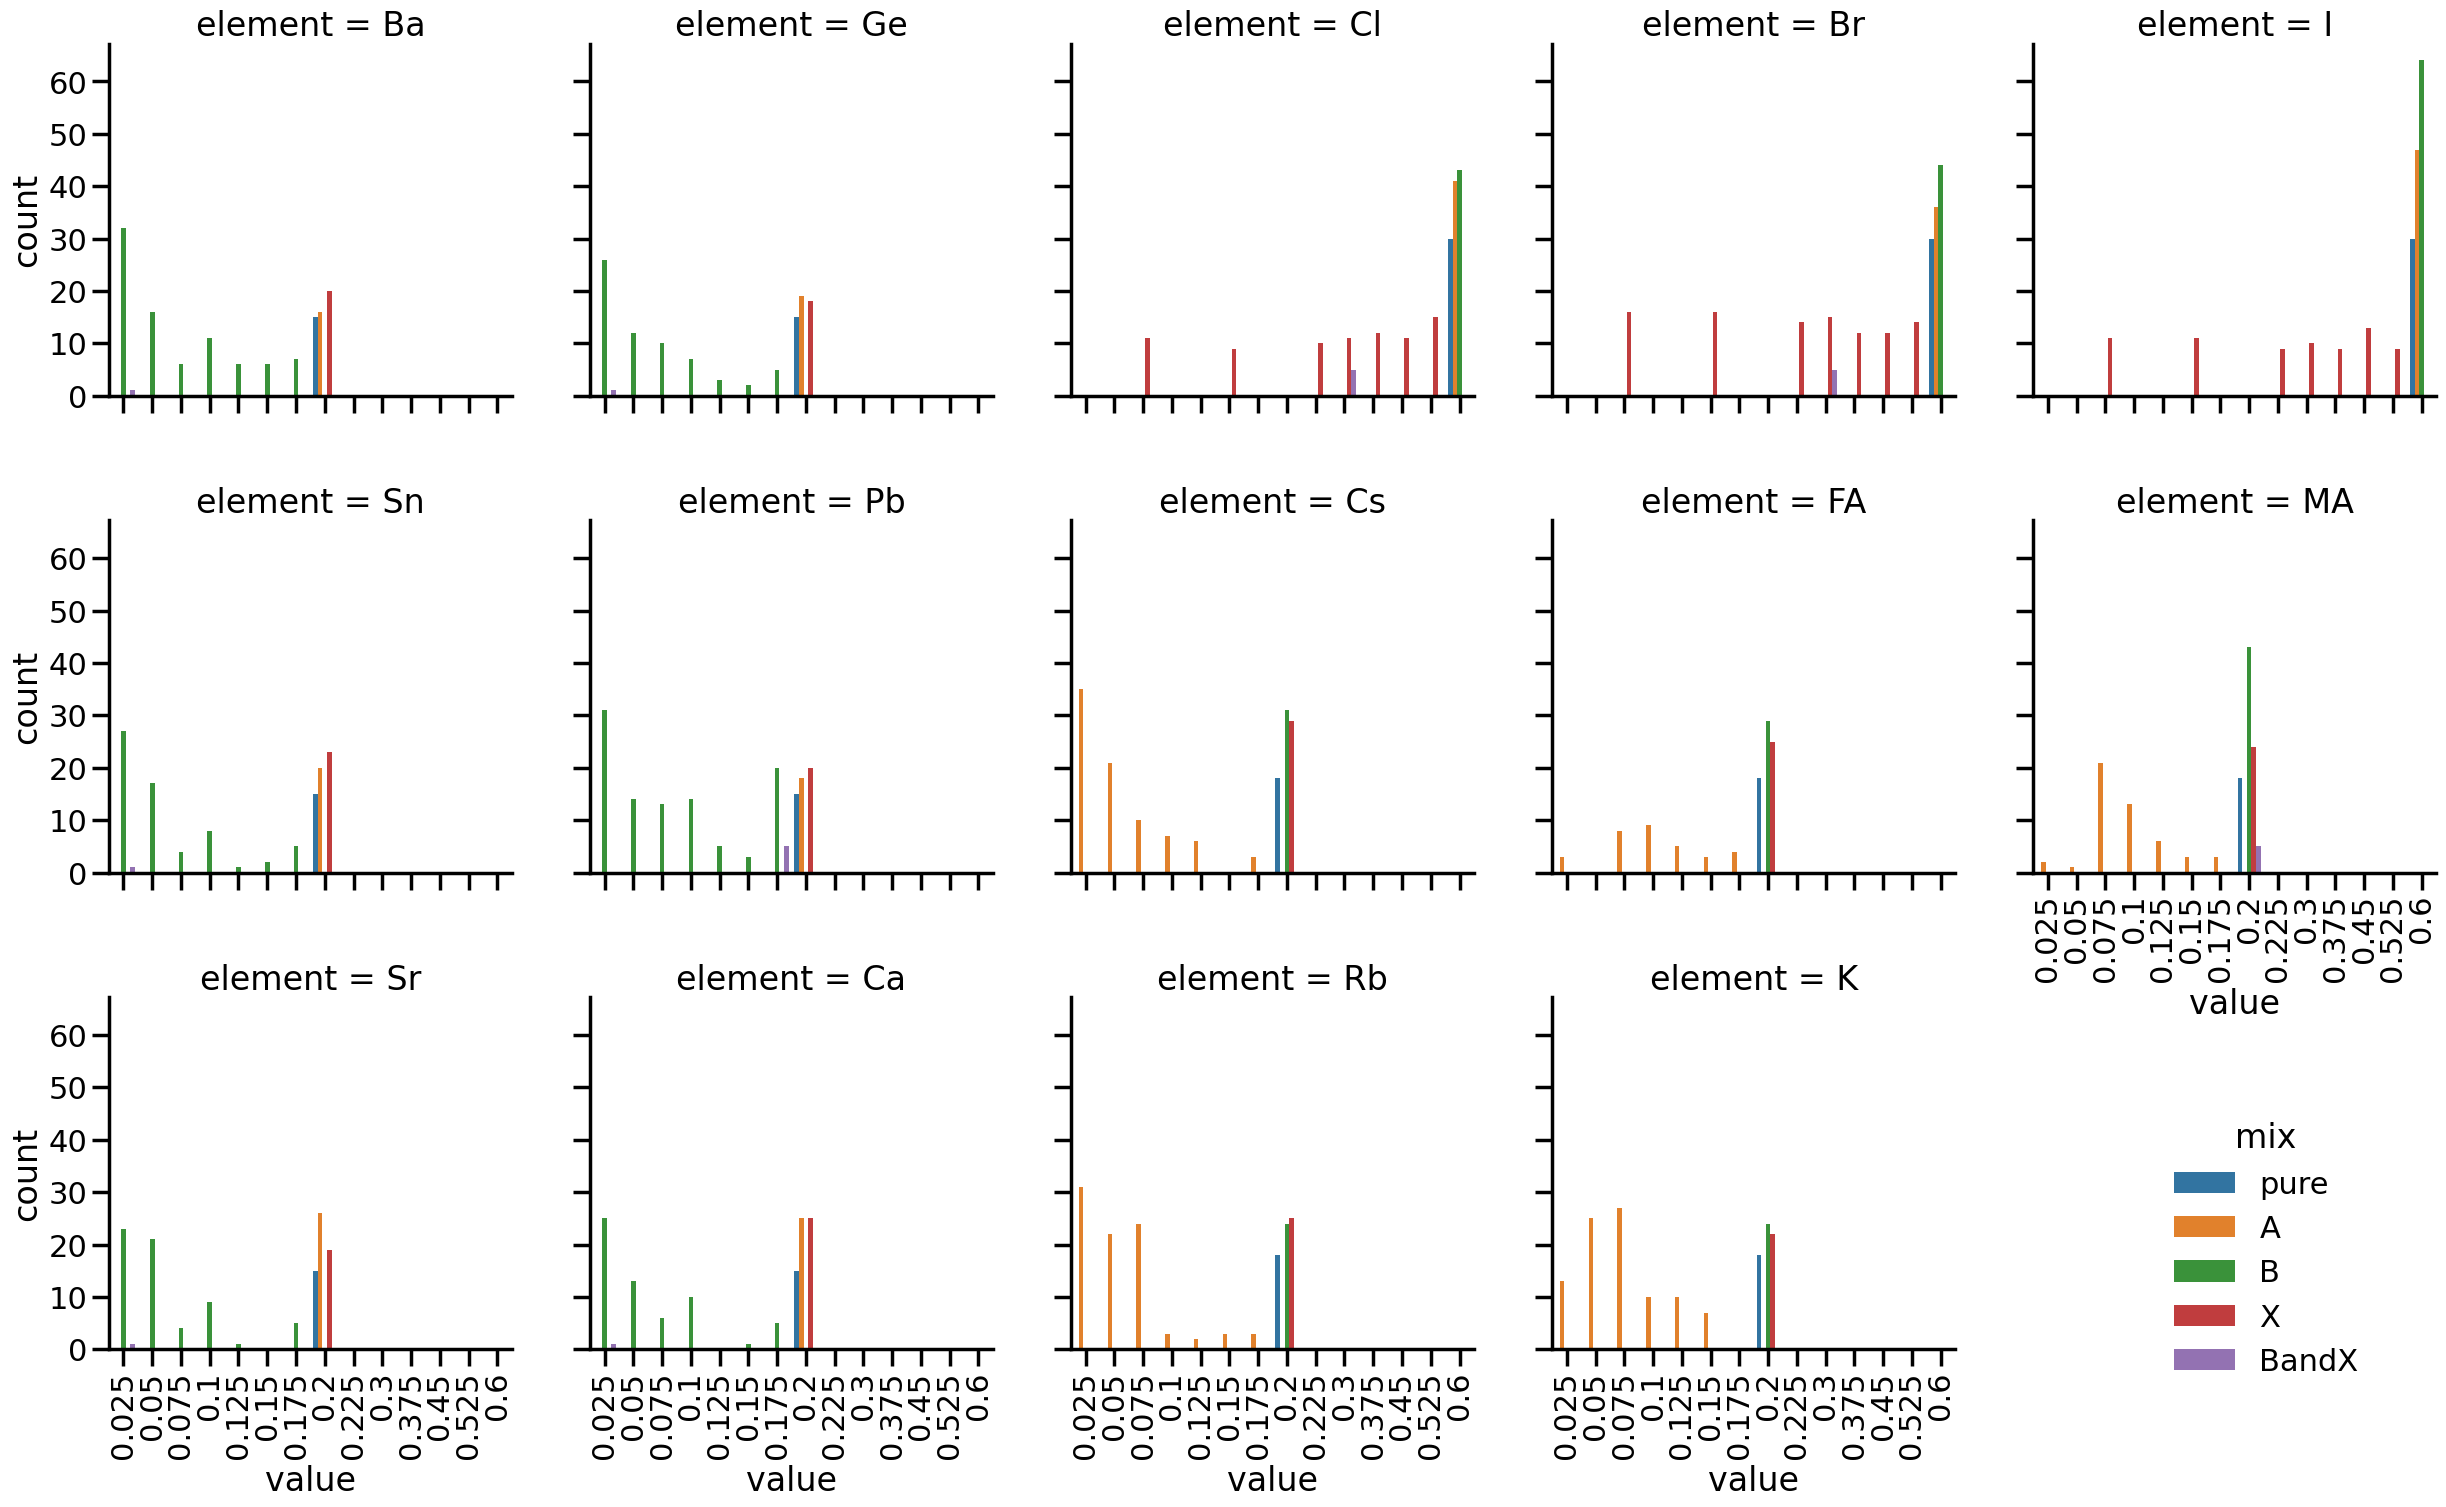
\includegraphics[width=.9\linewidth]{variability_of_composition_vectors.png}
\caption{\label{fig:chemspace_uni} Plots showing number of Perovskites representing a constituent at a certain atomic fraction of a complete Perovskite.}
\end{figure*}

\section*{Methodology}
\label{sec:orgd6791f9}
\subsection*{Building Perovskite Dataset}
\label{sec:org5d403ca}
The dataset we report is based on standard cubic phase ABX\textsubscript{3}
Perovskite structures obtained from public databases. Fourteen common
Perovskite constituents are selected to form our Halide Perovskite
composition space \ref{Fig:outline}. Five constituents including
Methylammonium and Formamidinium cations represent the possible A-site
occupants. Six heavy metal elements represent the possible B-site
occupants. Three halides represent the possible X-site occupants.

Each computational run is performed using a 2x2x2 supercell, this
allows A and B site doping to be modeled in discrete 1/8\textsuperscript{th} fractions
of the total site occupancy, and it allows X site doping to be modeled
in 1/24\textsuperscript{th} fractions. At this level, it is appropriate to call these
Perovskites alloys.

The pure (non-alloyed) possibilities are exhaustively sampled using 90
Perovskites. Based on these pure Perovskite structures, we mix
candidates for A, B, and X sites systematically. The alloy space sees
combinatorial scaling and must be sparsely sampled.

To create alloys, for example in B sites, we first select possible B
sites mixing elements.  Then SQS methods are applied to generate
random alloys for given mixing concentrations. Thus, we constructed
126 A-site mixing samples, 151 B-site mixing samples and 127 X-site
mixing samples. The resulting structures are optimized using a DFT
variable-cell relaxation.

\subsection*{Calculation Details}
\label{sec:orgba18d33}
Calculation DFT calculations are performed with Vienna Ab initio
Simulation Package (VASP) version 6.1. The projector augmented wave
(PAW) potentials were used The generalized gradient approximation (GGA)
of Perdew, Burke and Ernzerhof (PBE) and (HSE) is used as
exchange-correlation energy. The energy cutoff for the plane-wave basis
is set to 500 eV. The Brillouin zone was sampled by Monkhorst-Pack
k-point mesh, with a reciprocal mesh as 4x4x4. The structural force
convergence threshold is set to be 0.5 eV/Å.

\subsubsection*{LOPTICS Calculations and Absorption Spectrum}
\label{sec:org07dab61}

\subsection*{Analysis of DFT Computed Properties}
\label{sec:org40edc19}
\subsubsection*{Decomposition Energy}
\label{sec:orgbfed0ec}
The decomposition energy indicates the stability of a compound. To
calculate the decomposition energy for ABX3 perovskite, we assume it
will decompose to two phases, AX and BX2. Using DFT calculations, we
can get the optimized energy of a perovskite and that of its
constituent phases.

The equation is presenting the details calculation for decomposition
energy. For PBE decomposition energy, we use DFT energy results from
PBE level calculation. For HSE decomposition energy, we use the energy
from HSE level calculations.

\subsubsection*{Band Gap and Band Structure}
\label{sec:org967dddb}

\subsubsection*{SLME Package}
\label{sec:org48a51c1}
The SLME metric developed by \citet{yu-2012-ident-poten} is used as the
primary criterion screening perovskites for their photovoltaic
merits. The SLME value is computed for every Perovskite using Logan
William's SL3ME \cite{williams-2022-sl3me}.
\section*{Results and discussion}
\label{sec:org9bd497d}
\subsection*{Visualization of DFT Data}
\label{sec:orgf82c327}
\begin{figure*}
\centering
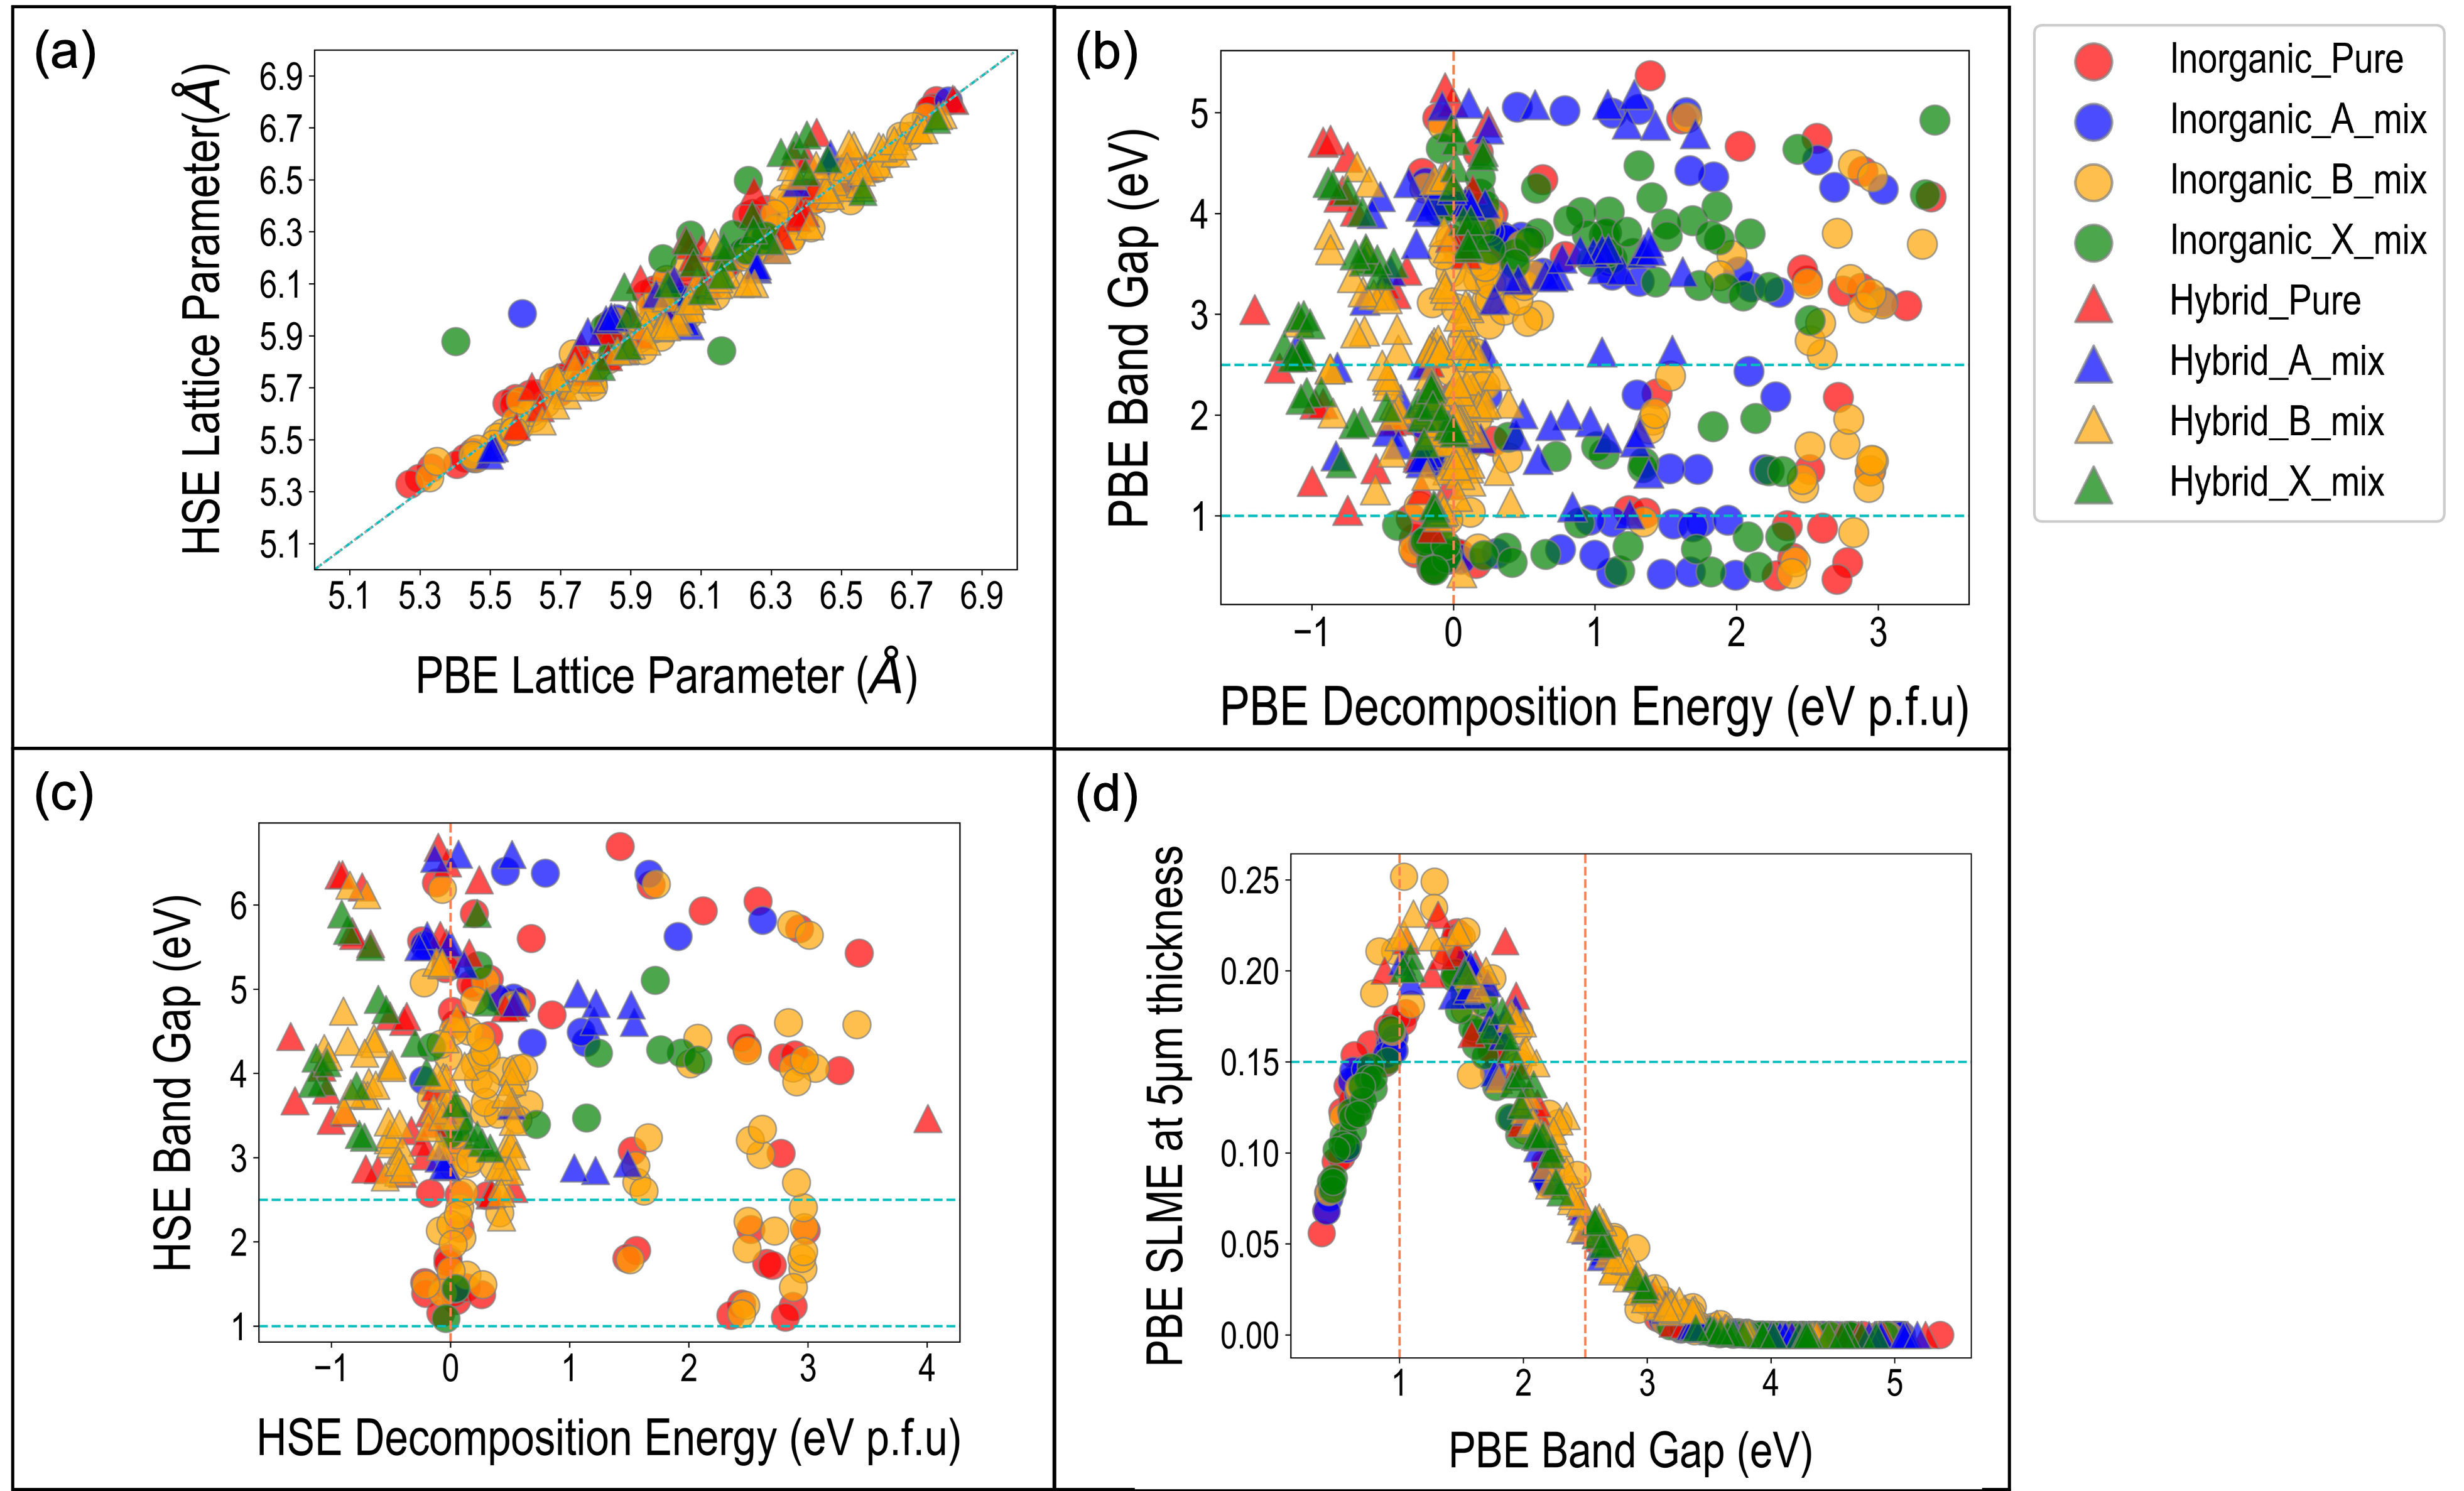
\includegraphics[width=.9\linewidth]{Figure2.png}
\caption{\label{Fig:pairplots} DFT Results: PBE and HSE properties; lattice constants, decomposition energies, band gaps, photovoltaic figure of merit.}
\end{figure*}

\subsubsection*{Lattice constant PBE vs HSE}
\label{sec:org2876770}
Fig 2(a) presents the lattice parameter comparison of PBE calculation
and HSE calculations. Most of the samples have close HSE lattice
parameters and PBE lattice parameters. This indicates that the accuracy
of PBE on lattice and structure is enough for most of the perovskite
samples. Some samples are observed significantly different lattice
parameters. By checking the optimized structures, we found that the
perovskite structure is largely deformed and no longer keep the
octahedral structures. Thus, we removed these 3 points for following
analysis.

\subsubsection*{Lattice constant vs experimental data}
\label{sec:org281c9b6}

\begin{figure*}
\centering
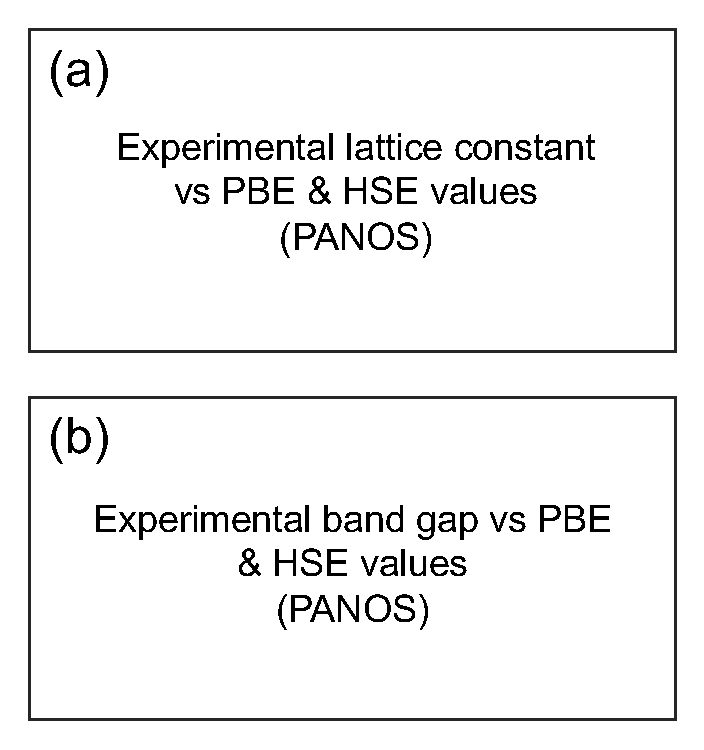
\includegraphics[width=.9\linewidth]{Figure3.pdf}
\caption{\label{Fig:lot_comp} Comparison of PBE and HSE computed properties with collected experimental measurements: (a) pseudo-cubic lattice constants, and (b) electronic band gaps.}
\end{figure*}

\subsubsection*{Decomposition energy vs band gap PBE and HSE}
\label{sec:orgc4e4e26}
Fig 2(b) is showing the PBE band gap compared to the PBE decomposition
energy. It presents the diversity of our perovskite dataset. The data
sets cover a large range of band gap and decomposition energy. For
example, we have perovskite with low decomposition energy (good
stability) and suitable band gap value (between 1 eV to 2.5 eV for PBE
calculations). And we can also find samples with low stability and large
band gap. The distribution of band gap and decomposition energy shows a
great diversity of all perovskite samples and indicates that our data
set can statistically represent a sufficient perovskite space. Fig 2(c)
shows the plot of HSE band gaps and HSE decomposition energy. Since we
applied HSE calculations for part of the samples, it shows some grouping
on low decomposition energy. Compared to PBE plot, more data should be
added in high decomposition energy region and suitable band gap region.

\subsubsection*{Spectroscopic Limited Maximum Efficiency (SLME) vs PBE Band gap}
\label{sec:org4847416}
Fig 2(d) presents the Spectroscopic Limited Maximum Efficiency (SLME)
values related to the PBE band gap. Spectroscopic Limited Maximum
Efficiency (SLME) is a very important properties for photovoltaic
performance. SLME measures the absorption efficiency of light for the
perovskite. As Fig 2(d) showing, a peak around 1.5 eV is obvious. The
peak indicates that these samples with 1.5 eV PBE band gap will also
have best absorption efficiency as photovoltaic materials. As the band
gap increases, the SLME value decreases and eventually goes to zero due
to the high band gap values.

\subsection*{Pearson Correlation Results}
\label{sec:org5c50364}
\begin{figure*}
\centering
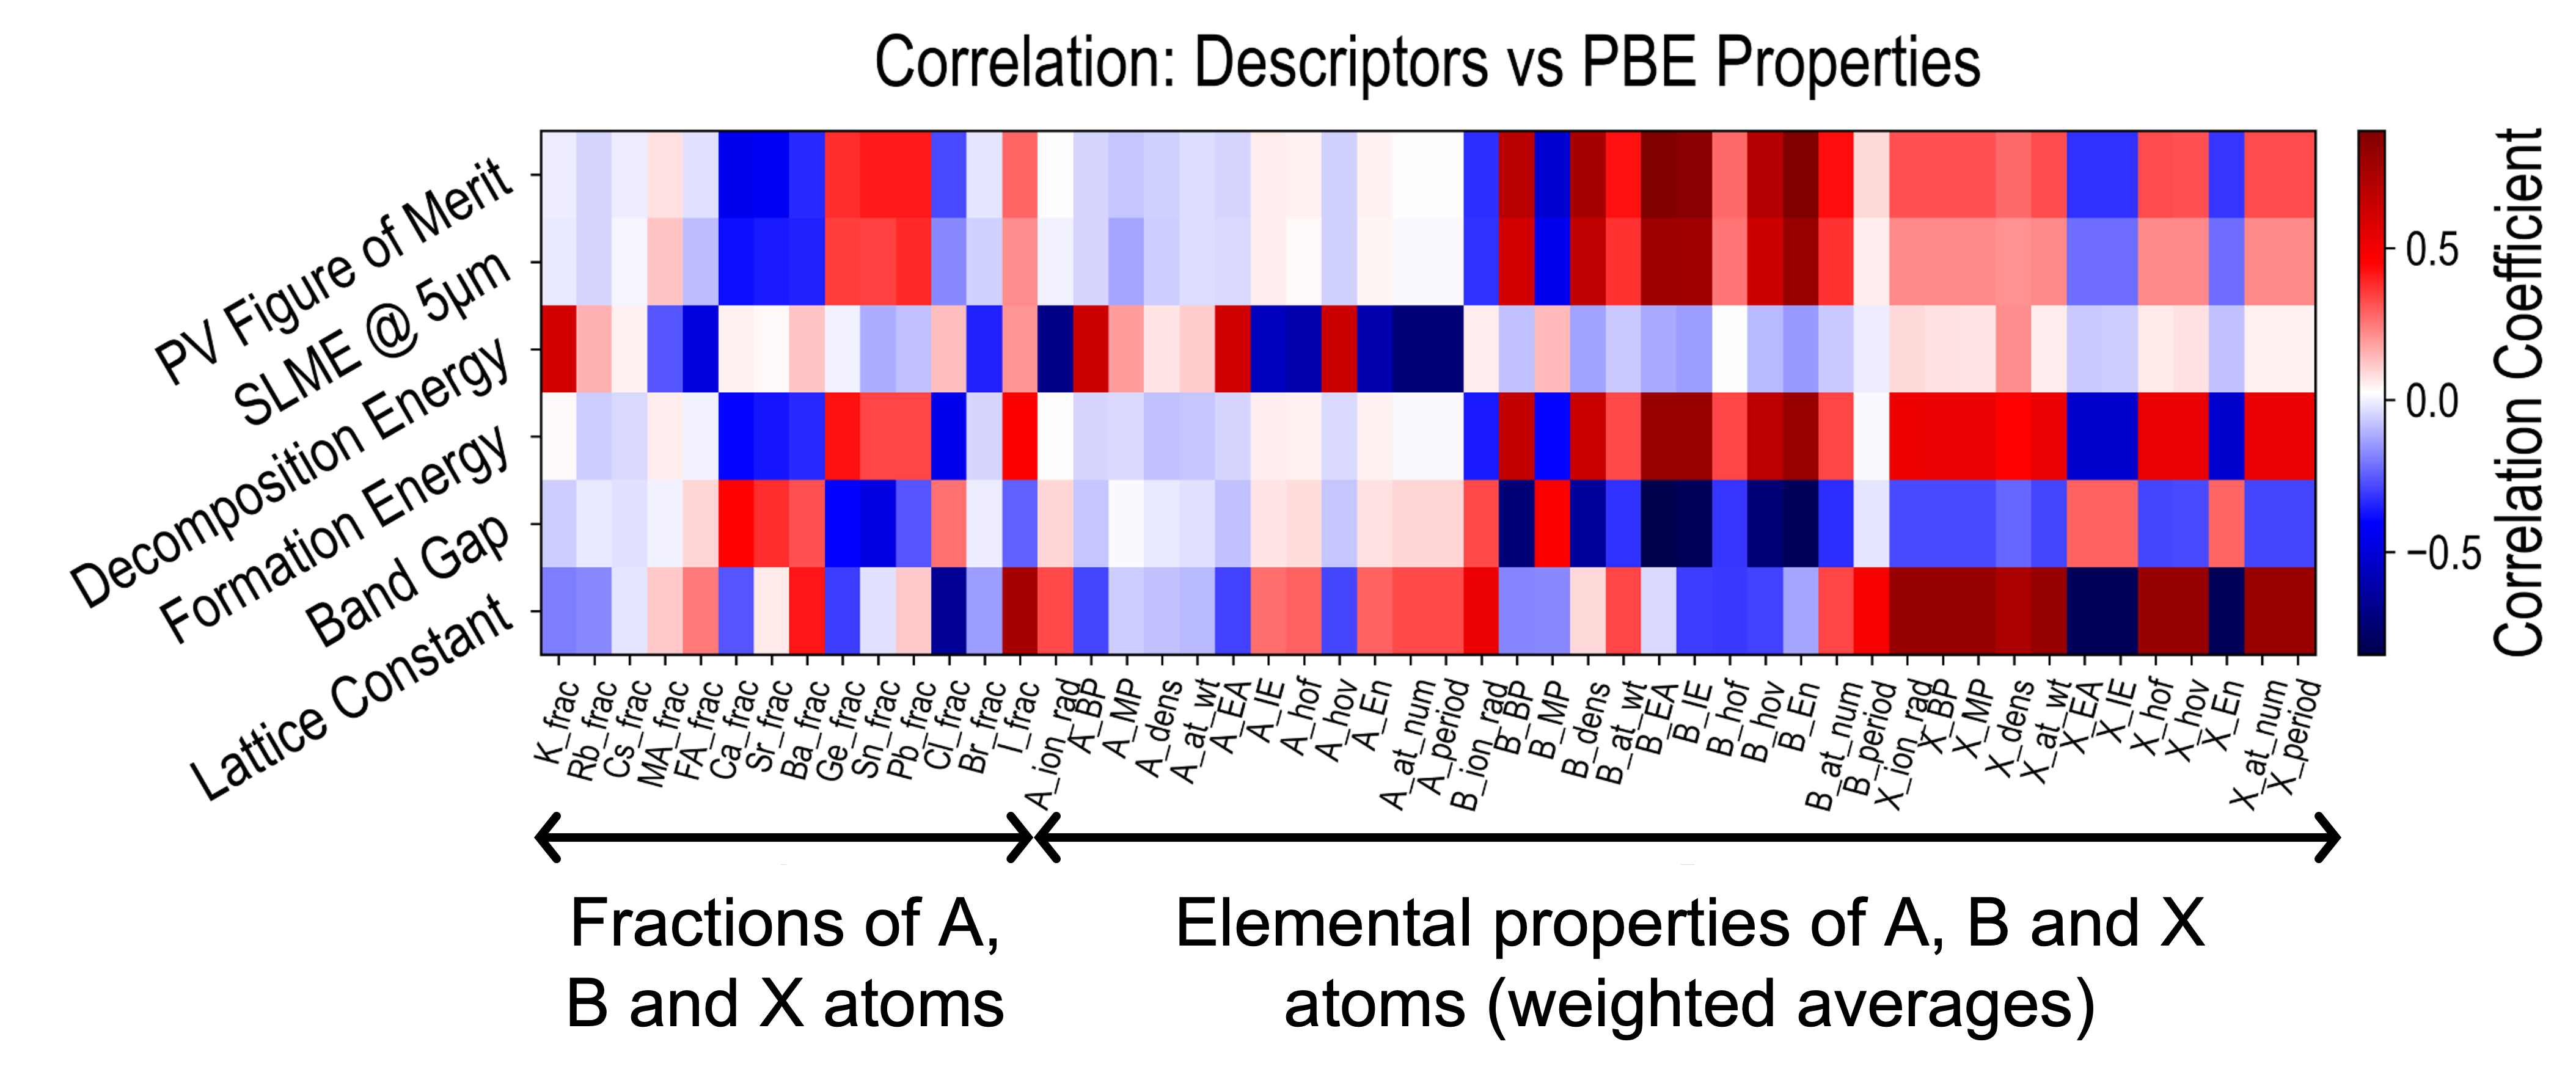
\includegraphics[width=.9\linewidth]{Figure4.png}
\caption{\label{Fig:pearson} Pearson linear correlation coefficients between 50 composition and elemental descriptors and (a) 6 PBE computed properties, and (b) 4 HSE computed properties.}
\end{figure*}

It is unlikely that any of the targets is fully explained by a single
composition or composition derived axis. But there are helpful relations
that aid in obtaining a physical understanding.

as in a Pearson correlation map is produced to check for strong
relations. Those that exist, when plotted in detail show some trending,
but always with extensive variability. Evidently, an accurate model will
have to be formed on a multidimensional domain.

\subsection*{PCA}
\label{sec:org9c06e77}
\begin{figure*}
\centering
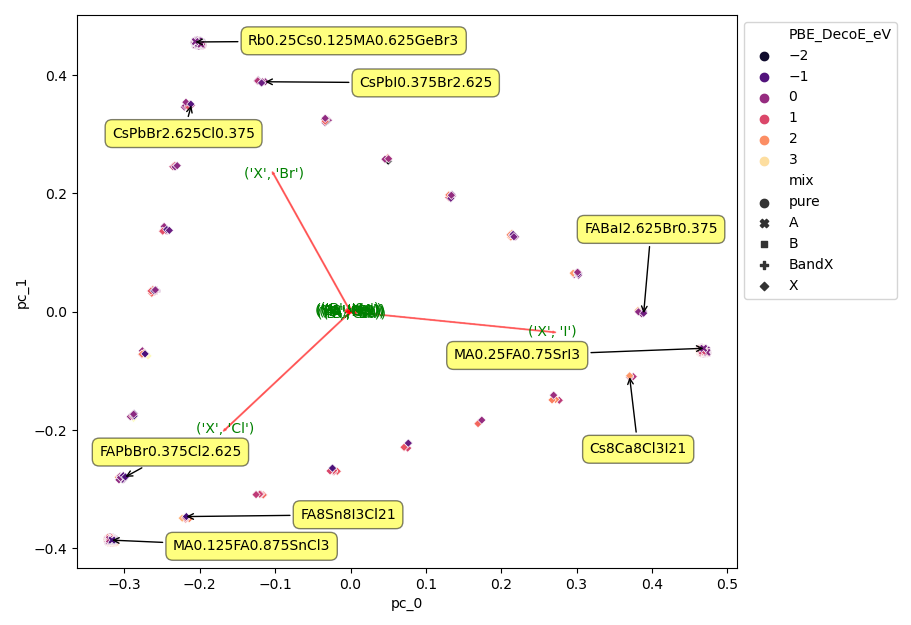
\includegraphics[width=.9\linewidth]{comp_ratio_projection_annot.png}
\caption{\label{Fig:pca} PCA}
\end{figure*}

Principal Component Analysis is a method of projecting high dimensional
data onto a plane defined by the two linear combinations of axes that
explain as much of the variance as possible.

The method of PCA is the Singular Value Decomposition, a Unitary
Transform which generalizes the familiar eigendecomposition. PCA will
"rotate" the N data points in M-D space until their widest 2D cross
section is displayed.

At this point it is readily apparent that this dataset is highly
topological. The data exists on a mostly bounded domain in high
dimensions, so there is some geometry the features constitute.

Our models will prefer to use this this geometric structure in their
explanation for why perovskite properties vary, this can be useful for
accuracy, it can also be a bias-inducing hindrance.

\subsection*{MDS / T-SNE / Isomap Results}
\label{sec:org413ea63}

\section*{Perspective and Future Work}
\label{sec:orgd51dc43}
The design of this dataset is uniquely suited to the exploration of
alloying effects on Perovskite properties. The combinatorial space of
possible alloys has been sparsely but systematically sampled along
four primary alloy schemes. This sample space affords the opportunity
for a QM/ML surrogate model to form the basis of an active learning
strategy which can begin selecting potentially high performing
multi-site alloy candidates based on the current sample set.

The principal challenge will be in extracting features useful as
performance features. The basic feature sets examined here are highly
correlated, but nonetheless show promise as basic screening criterion.

Modeling pipelines capable of predicting Perovskite decomposition
energy will likely be very achievable using a transductive and
invertible equivalent of the tSNE algorithm, potentially SONG.

\section*{Conclusions}
\label{sec:orgc2e1771}
\ldots{}\\

\section*{Conflicts of interest}
\label{sec:orgb4090d0}
There are no conflicts to declare.

\section*{Acknowledgements}
\label{sec:org2407fa5}
Extensive discussions with and scientific feedback from UC San Diego
researchers David Fenning and Rishi Kumar and Argonne National Lab
scientist Maria Chan are acknowledged. This work was performed at Purdue
University, under startup account F.10023800.05.002 from the Materials
Engineering department. This research used resources of the National
Energy Research Scientific Computing Center, the Laboratory Computing
Resource Center at Argonne National Laboratory, and the RCAC clusters at
Purdue.

\bibliographystyle{rsc}
\bibliography{../../../org/bibliotex/bibliotex}
\section*{Supplemental Material}
\label{sec:org38d596a}
\end{document}